% Code from Christian Feuers??��nger
% http://tex.stackexchange.com/questions/54794/using-a-pgfplots-style-legend-in-a-plain-old-tikzpicture#54834

\documentclass{standalone}

\usepackage{tikz}
\usetikzlibrary{shapes, positioning, calc}

\begin{document}
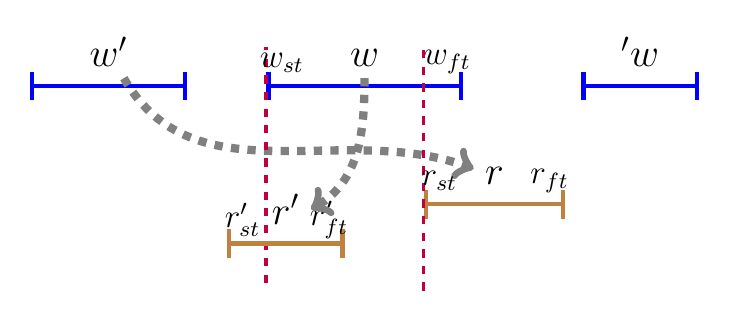
\begin{tikzpicture}[]

% new command: inverval
\newcommand{\itv}[4] % #1: start point; #2: end point; #3: operation name; #4: color
{
  \coordinate (start #3) at #1;	% start point
  \coordinate (end #3) at #2;	% end point
  % \coordinate (mid) at ($0.5*#1 + 0.5*#2 + (0,0.8cm)$);

  \draw[ultra thick, #4, |-|] (start #3) -- (end #3) % draw the interval
    node[pos = 0.5, above = 1mm,font = \Large, text=black] (#3) {$#3$}; % attach the operation name
  % \node (#3) [font = \huge] at (mid) {$#3$};	% attach the operation name
}

\begin{scope}[]
  % \itv{(-2,0)}{(-0.5,0)}{w''}{blue}
  \itv{(-1,0)}{(1,0)}{w'}{blue}
  \itv{(2,0)}{(4.5,0)}{w}{blue}
  \itv{(6.0,0)}{(7.5,0)}{'w}{blue}

  \itv{(4.0,-1.5)}{(5.8,-1.5)}{r}{brown}

  \draw [dashed, line width = 3pt, gray, ->] (w') to [out = -60, in = 160] (r);

  % concurrency interval
  \draw [purple, dashed, very thick] ($(start r) + (0,-1.1)$) to ($(start r) + (0,2)$);
  \draw [purple, dashed, very thick] ($(start w) + (0,-2.5)$) to ($(start w) + (0,0.5)$);

 % reads finish in the concurrency interval
  \itv{(1.5,-2)}{(3.0,-2)}{r'}{brown}
  % \itv{(1,-2.0)}{(3.5,-2.0)}{r'}{brown}


  % starting time and finish time for r, w, and w'
  \node [font = \large] at ($(start r) + (0.2,0.3)$) {$r_{st}$};
  \node [font = \large] at ($(end r) + (-0.2,0.3)$) {$r_{ft}$};

  \node [font = \large] at ($(start w) + (0.2,0.3)$) {$w_{st}$};
  \node [font = \large] at ($(end w) + (-0.2,0.3)$) {$w_{ft}$};

  \node [font = \large] at ($(start r') + (0.2,0.3)$) {$r'_{st}$};
  \node [font = \large] at ($(end r') + (-0.2,0.3)$) {$r'_{ft}$};

% reads returning the latest value
\draw [dashed, line width = 3pt, gray, ->] (w) to [out = -90, in = 30] (r'.east);
\end{scope}

\end{tikzpicture}
\end{document}
